\chapter{Overall description}
\section{Product perspective}
Data4Help will be a service accessible through a web application for third parties and through a smartphone application for individuals. These application will be completely developed ground up, while for some backend and critical activities, external software will be used in order to speed up the development.


The following class diagram helps to visualize how Data4Help will try to provide services for both the individuals and the third parties by functioning as a central hub of eHealth data

\begin{figure}[H]
  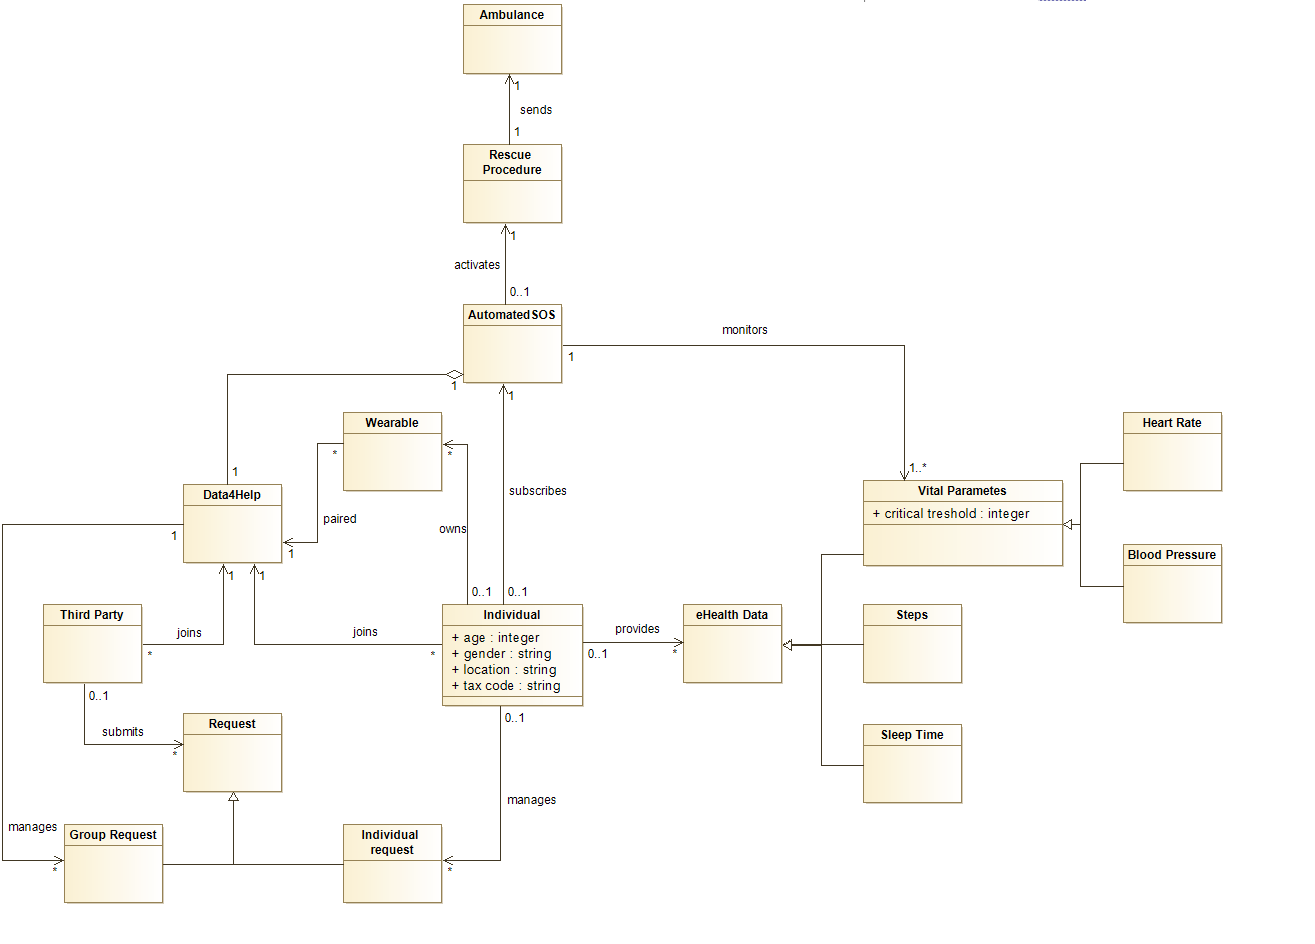
\includegraphics[width=0.89\linewidth]{resources/UML/Data4HelpClassDiagram.png}
  \caption{Data4Help Class Diagram}
  \label{fig: Data4Help Class diagram}
\end{figure}

Regarding the AutomatedSOS service, the following statechart diagram describes what are the main phases of this service

\begin{figure}[H]
  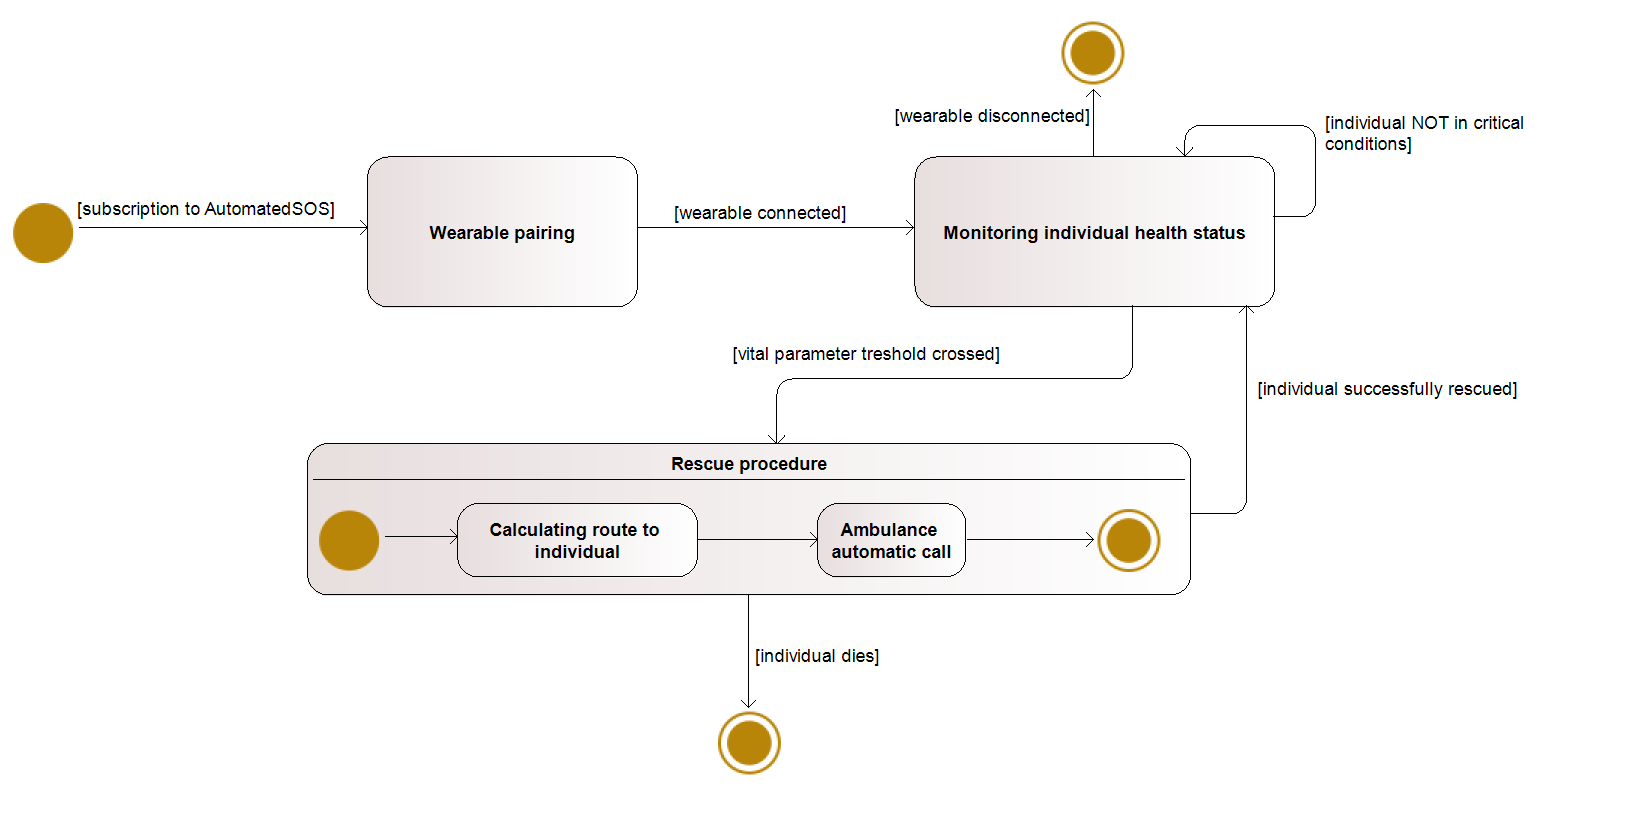
\includegraphics[width=0.89\linewidth]{resources/UML/AutomatedSOSstatechart.png}
  \caption{AutomatedSOS statechart diagram}
  \label{fig: AutoamtedSOS statechart diagram}
\end{figure}


\subsection{Access to specific data}
A third party interested in monitoring a specific individual can send a request to the system specifying his SSN, TC or his username.
The system passes the request to the specific individual who can accept or refuse it.
Once the individual has given an answer, the system notifies the third party about the answer: if the individual has given the consent to access his data the third party can then visualize the data.

The data access permission can be managed by the indivudals through their application, and can be removed anytime from when it was accepted. 
In this case the third party is notified about the individual decision and should formulate another request in order to access again individual's data. 




\subsection{Access to group data}
A third party can also request access to anonymized data of a group of individuals.
To do so, it must specify some parameters concerning individuals. These parameters can regard geographical area, age range or level of education of the users of interest to the third party.
Geographical area can be specified in term of country, region, province, town and district (only for big city).

This type of requests are managed directly by the system. Because TrackMe holds in high regard the privacy of its users, it will satisfy the request only if the number of individuals whose data satisfy the request is higher than 1000.

If the request is positively evaluated, the anonymized data is made available to the third party.
Optionally, the third party can subscribe to new data with the same characteristics. If new data, matching the third party request, is produced it will be made available to the requester at most once a week.

\subsection{Data Subscription}
Third parties can optionally subscribe to data of accepted requests: if new data, matching the third party request, is produced then it will be notified made available to the requester at most once a week.

The data is provided as long as the data request is valid: if the number of individuals that are part of a grpup request goes to 1000 or less, or the individual removes the data access the system stops to update the third parties. 

Third parties can at any moment,from the subscription to a data request, unsubscribe.





\subsection{SOS service}
The service AutomatedSOS must exploit the real-time stream of eHealth data provided by the underlying Data4Help to offer a personalized and non-intrusive SOS service especially designed for elderly people.
Any individual, correctly registered to Data4Help, can optionally request to active this service


If AutomatedSOS has been activated, the system should continuously monitor the parameters of the individuals and compare them using certain specific thresholds.
If the parameters are below these thresholds, the system assumes that the individual is having a sudden illness and forwards a request to an emergency service for sending an ambulance to the location of the user.
AutomatedSOS must ensure a reaction time of less than 5 seconds from the time the parameters are detected below the threshold.










\section{User characteristics}
The users of Data4Help and AutomatedSOS services are:

\begin{itemize}
\item \textit{Individual} : user that allows the acquisition of the data and can optionally activate AutomatedSOS. He can't use the data request feature of Data4Help.
\item \textit{Third party}: user that can request data from the application.
\end{itemize}





\section{Assumptions, dependencies and constraints}

\subsection{Domain assumptions}

\begin{itemize}


\item[] \dom{ 
Location and eHealth data are provided by individuals' devices and assumed to be correct.
}{ProvidingData} 
\item[]\dom{
A third party interested in monitoring a specific individual knows the SSN of the individual
}{SSNknown}
\item[]\dom{
Users have access to internet.
}{Internet}
\item[]\dom{
Thresholds for health parameters are provided by medical experts.
}{Tresholds}
\item[]\dom{
An ambulance is always available when it is needed.
}{Ambulance}
\item[]\dom{
Registered users must keep their login credentials secret.
}{Credential}
\item[]\dom{
The ambulance driver can reach the user in critical condition.
}{Reachability}
\end{itemize}




\subsection{Privacy constraints}
The system will collect and elaborate personal data of the individuals and, possibly, it will share them or part of them with third party.  For this reason, during the registration activity to the system, all the users must be informed of this practice and they must explicitly confirm their consensus.

In particular, anonymized data can be shared with third parties who request it without the users being further advised. In order to protect its users' privacy and to prevent misuse of data, TrackMe won't share data if the number of individuals whose data satisfy the request is lower than 1000.

Moreover, a third party can request to fully access the data of some specific individual. In this case it is up to the individual to accept or not to share his data with that specific third party.


